\chapter{Background}\label{cp:theory}
This chapter discusses the findings of researching existing and proposed algorithms for determining systolic and diastolic blood pressure through the oscillometric method. This report focusses on relatively simple algorithms that can be implemented in a real-time application, which is the goal of this project.

The first part of this chapter defines what blood pressure is and how it is measured manually. Afterwards, different algorithms are explained and examined. 

A section at the end of this chapter explores algorithms beyond the scope of the project that have been proposed in recent literature.

\section{What is Blood Pressure?}

Blood pressure is an essential bio-medical measurement and often used for diagnostics in cardiovascular diseases. Most commonly, systolic and diastolic blood pressure are mentioned in pairs, but what do those mean?

The heart is a pump that has two phases. When the ventricle is relaxed, the heart fills up, and the diastolic blood pressure (DBP) is observed. When the heart contracts, it pushes the blood through the arterial system, and the systolic blood pressure (SBP) is observed. A third characteristic is the difference between SBP and DBP, the pulse pressure (PP). Finally, the mean arterial pressure (MAP) is defined as the average pressure in the artery. Figure \ref{fig:BP} shows how these pressure values are connected in two heartbeats. MAP is the area underneath the blue curve divided by the time of one pulse, indicated by the orange area \citep{Boron2012}. Because blood pressure is simplified as a sine wave, the MAP is in the middle between SDP and DBP. Usually, the MAP is closer to DBP. \paragraph{}


\begin{figure}[ht]
\centering
\includegraphics[width=0.65\textwidth]{figures/MAP1.pdf}
\caption{Characteristic blood pressure values simplified as a sine wave. The values are: MAP: \SI{100}{\mmHg}, SBP: \SI{120}{\mmHg}, DBP: \SI{80}{\mmHg} and heart rate: \SI{60}{beats\per\second}.}
\label{fig:BP}
\end{figure}

Blood pressure can be measured with invasive and non-invasive methods. The most accurate technique is invasive and requires professional expertise because a catheter has to be injected into the blood vessel \citep{Boron2012}. Subsequently, non-invasive methods are more common because they are more convenient to use. With automated means, taking blood pressure at home has become comfortable and straightforward. However, the inaccuracies of these measurements are often ignored or even unknown.

\section{Manual Blood Pressure Measurement}
The manual method of measuring blood pressure relies on a sphygmomanometer and listening to the heart or Korotkoff sounds (named after their discoverer) with a stethoscope. This is called the \emph{auscultatory method}. \emph{Palpation} is another method where the pulse is felt at the wrist. It only allows detection of the SBP. The auscultatory method is described below because it provides recommendations that are true for all blood pressure measurements using a cuff.

A sphygmomanometer is shown in figure \ref{fig:sphy}. It consists of an inflatable cuff, connected to a rubber pump and a scale that indicates the pressure in the cuff in \SI{}{\mmHg}. The pump is equipped with a valve that can be opened to release air.

Millimetres of mercury (\SI{}{\mmHg}) is a unit to describe pressure. \SI{1}{\mmHg} is defined as the pressure generated by a column of mercury of \SI{1}{\mm} height. Millimetres of Mercury is not part of the International System of Units (SI) but was defined by it before 2019 as \SI{1}{\mmHg} = \SI{133.322}{\Pa} using standard gravity \citep{SI2006}. Since 2019, \SI{}{\mmHg} is no longer included in the SI brochure. However, it is still widely used in the medical field \citep{Prazak2020}.

\begin{figure}[h]
\centering
%\includegraphics[scale=0.125]{figures/spy.pdf}
\caption{Picture of a sphygmomanometer showing the cuff, inflation pump and mercury meter.}
\label{fig:sphy}
\end{figure}

Intra-arteria or direct BP measurement is considered the 'gold standard', but most studies compare the developed algorithm with the auscultatory method, which underestimated SBP and overestimates DBP. according to \citet{Sapinski1996}. Nonetheless, the protocols to test automatic blood pressure monitors given by the British Hypertension Society (BHS) and their American counterpart, the Association for the Advancement of Medical Instrumentation (AAMI), both use the auscultatory method as a reference \citep{Jazbinsek2010,OBrien1993,AAMI2013}.

\subsection{Auscultatory Method}
The cuff size must be appropriate for the patient's arm. The rubber bladder inside the cuff should cover more than \SI{80}{\%} but less than \SI{100}{\%} of the arm's circumference.

The cuff is completely deflated and tightly fit around the upper arm of the patient. The centre of the bladder should be over the brachial artery and the arm supported at heart level. The stethoscope is to be placed over the artery between the cuff and the patient's elbow and should not touch the cuff. The stethoscope being pressed on the arm could influence the reading because it puts additional pressure on the artery and can interfere with hearing the sounds.
The valve at the pump is completely closed. Then the cuff is inflated to a pressure of about \SI{30}{\mmHg} above the expected systolic pressure. That causes the artery to flatten and not let any blood through. Next, the valve is slightly opened to slowly deflate the cuff at a rate of approximately \SI{3}{\mmHg/\second}. The artery will open and let small amounts of blood through. Systolic pressure is read when a pulse is first heard. Meanwhile, deflation continues. Diastolic pressure is read when the sounds disappear entirely. Ultimately, blood can flow freely through the artery. After making sure that no further sounds can be heard by deflating for at least another \SI{10}{\mmHg}, the valve is opened completely to empty the cuff. \citep{Lloyd2018, Reeves1995}

There are some discrepancies in literature ton how to define the point of the diastolic blood pressure. Some references define it as when the Korotkoff sounds disappear entirely \citep{Lloyd2018, Reeves1995}. Others describe it as the point where the sounds are muffled \citep{Boron2012}. Here, the former is assumed, because most current literature does and some research suggests that the auscultatory method overestimates diastolic blood pressure \citep{Chandrasekhar2019}.

\subsection{Calculation of MAP}
Traditionally, MAP is calculated as an estimate by adding a third of the PP to the DBP. Or, how it is more commonly referred to, adding SBP and twice the DBP and dividing the result by three (equation \ref{eq:MAP}). According to calculations by \cite{Bos2007}, this underestimates the MAP, and they suggest to add $40\%$ rather than a third of DBP. Furthermore, they propose to use MAP measured by oscillometric devices rather than calculating it from values obtained through the auscultatory method. 

\begin{equation}
\label{eq:MAP}
MAP = \frac{SBP-DBP}{3}+DBP = \frac{SBP+2\times DBP}{3}
\end{equation}

As explained by \cite{Joe2019}, nurses in intensive care units (ICU) today still use the manual calculation method on the automatically obtained SBP and DBP rather than rusting the measured MAP, which introduces significant errors.

\section{Automatic Blood Pressure Measurement}
Most modern automatic devices use the oscillometric method to determine blood pressure. They are used both at home and in professional environments.

Automatic blood pressure monitors measure pressure in a cuff similar to the one used in the manual method. It uses the small pressure changes (oscillations) extracted from the deflation curve to estimate blood pressure. Commercially available devices are usually equipped with an electric pump, and the bladder contains a pressure sensor. Otherwise, they look similar to the cuff used for manual measurements. Some devices use wrist cuffs, but those are rarely recommended \citep{BIHS2020}. The most significant problem using wrist measurements is the influence of gravity on blood pressure and the accompanying risk of systematic errors when the device is not at heart level \citep{Boron2012}. This problem is avoided by taking blood pressure at the upper arm.

\paragraph{General Procedure} The procedure is likewise similar to the manual method. Pressure in the cuff is increased to a level above the expected systolic pressure, which leads to the artery being pushed close. While releasing the air slowly through the valve, blood starts flowing through the artery, resulting in small increases in pressure relative to the continued deflation of the cuff. As the cuff deflates further, these relative changes increase to a maximal value before they start decreasing again \citep{Forouzanfar2015, Drzewiecki1994, Ursino1996}. The shape, magnitude or envelope of these oscillations are used in various automatic blood pressure algorithms. Methods that do not use oscillations exist, but are not discussed here. 


\paragraph{Oscillation Extraction} There are two ways the oscillometric waveform (OMW) is extracted from the deflating pressure curve. The first one is filtering. A bandpass filter with a lower cut-off frequency between \SIrange{0.1}{0.5}{\Hz} and an upper cut-off frequency between \SIrange{5}{20}{\Hz} is recommended \citep{Forouzanfar2015}. Implementations usually use first \citep{Lim2015} to sixth order \citep{Jazbinsek2010} Butterworth filters. They are known for their flat pass-band response and good frequency response. 

The second approach is to use detrending. It requires to know the beginning of each pulse to be able to fit a line of continuously deflating pressure to the identified points. Its advantage is, it additionally reproduces an estimated deflation curve. However, it requires additional data, for example, ECG for pulse detection \citep{Forouzanfar2015}.

\begin{figure}[h]
\centering
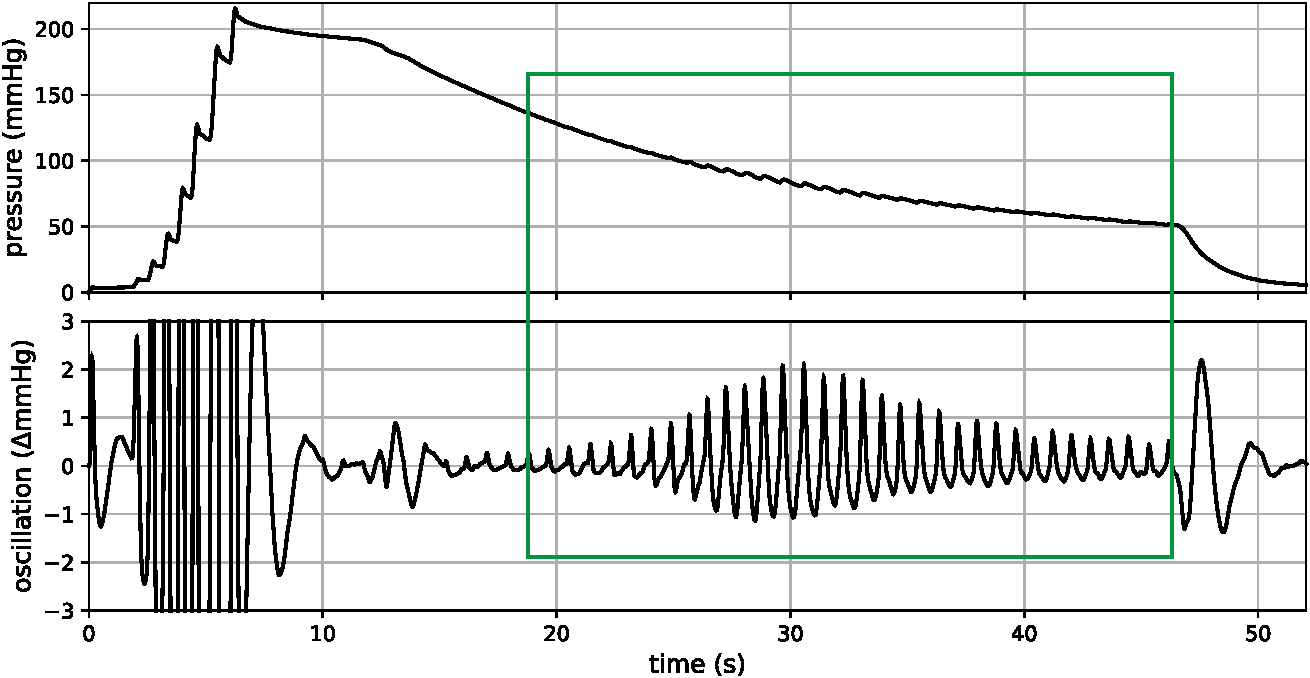
\includegraphics[width=0.95\textwidth]{figures/sample_data.pdf}
\caption{The deflating pressure data in the top plot is filtered with a \nth{4} order Butterworth high-pass filter with the cut-off frequency at \SI{0.5}{\Hz} to extract the oscillations. The rectangle highlights the vital part of the data.}
\label{fig:osc}
\end{figure}


Ultimately, from a deflation curve as in the signal in figure \ref{fig:osc} on the top, the oscillations are extracted. The bottom plot in figure \ref{fig:osc} shows oscillations extracted with a \nth{4} order Butterworth high-pass filter with the cut-off frequency at \SI{0.5}{\Hz}. The rectangle shows the part of the signal that is analysed further.


\paragraph{Envelope} 
Basic automatic algorithms use the OMW envelope (OMWE). Formation of the envelope is achieved in different ways. The simplest is to register only local maxima. Similarly, and most common, are the subtraction of the following through from a local peak or interpolating the curve of local maxima and local minima to subtract them from each other. Some algorithms additionally fit a curve on the obtained OMWE in an attempt to remove artefacts \citep{Forouzanfar2014}.


\subsection{Maximum Amplitude Algorithm}\label{sec:MAA}
The maximum amplitude algorithm (MAA) is based on the assumption that the oscillations are maximal when the pressure in the cuff equals arterial pressure. Accordingly, the recorded pressure at which oscillations are maximal is considered a valid estimate of the MAP \citep{Babbs2012, Geddes1982, Drzewiecki1994, Ramsey1979}, as long as the compression chamber is kept small \citep{Mauck1980}. The cuff should always be tightly fit, to avoid introducing errors. Air in the cuff causes maximum oscillations to be above the accurate MAP. Hence, Ursio and Cristalli suggest using the lowest pressure of the plateau of maximal oscillations as the value to assess MAP \citep{Ursino1996}.

The publication by \citet{Chandrasekhar2019} employs a more complex model than the one initially introduced by \citet{Mauck1980}. They conclude that the MAA results in a weighted average of systolic and diastolic BP. According to their model, MAA underestimates MAP for higher blood pressure.

\paragraph{Fixed-Ratio Algorithm} The fixed-ratio algorithm builds on the MAA. It is based on the assumption that the systolic and diastolic blood pressure occur at specific fractions of the maximum oscillation before and after its occurrence. Determining SBP and DBP after applying the MAA was tested by \citet{Geddes1982}. They recorded the Korotkoff sounds while measuring oscillations to find a ratio of amplitudes for SBP and DBP. They defined the coefficient for the systolic pressure to be 0.5 and the one for the diastolic pulse as 0.8. These ratios were found empirically, and Geddes acknowledges that the systolic pressure is overestimated and the ratio for the diastolic pulse is not constant for a range of different diastolic pressures.

Later studies tried to find accurate ratios, mostly experimentally with the ratio for SBP usually being determined between 0.45 and 0.73 and the ratio for DBP a bit higher between 0.69 and 0.83 \citep{Drzewiecki1994, Forouzanfar2015}. Mathematical models confirmed that a generalised ratio could not be found. Parameters like the age of the subject, the arterial stiffness and pulse pressure influence the ratios \cite{Ursino1996}. A higher PP results in a smaller ratio for SBP and larger ratio for DBP. A stiff arterial wall causes volume changes to happen slower. While this has little effect on the systolic ratio, the diastolic ratio decreases with the stiffness of the artery \citep{Babbs2012}.

\subsection{Derivative Algorithm} \label{sec:der}
The derivative algorithm uses the OMWE and plots it against the deflation pressure. Next, the points of the maximal and minimal slope are determined. The pressure point where the derivative of the OMWE is maximal is assumed to be the diastolic BP and where the derivative is minimal is the systolic BP, respectively \citep{Jazbinsek2010, Forouzanfar2015}.

Even though mathematical models have confirmed this method to produce valid estimates of both SBP and DBP without the need for empirically obtained ratios, it is exceptionally vulnerable to noise and therefore not used in practical applications \citep{Babbs2012, Chandrasekhar2019}.

\citet{Jazbinsek2010} evaluated the fixed-ratio and derivative algorithm. They used a device equipped with an electrocardiogram (ECG) and a microphone to validate their results. Various ways to form the envelope were used, including detrending, filtering and even using the low-frequency part of the audio signal of a microphone that recorded Korotkoff sounds. However, to evaluate the fixed-ratio method, they used a commercial device to find average ratios and used the values from the same tool as a reference for the evaluation. As was to be expected, their implementation of the derivative algorithm showed many local extrema. The algorithm was only able to perform by applying additional constraints that bias the measurements significantly. For example, the extrema have to be distanced from the MAP value more than \SI{15}{\mmHg} \citep{Jazbinsek2010, Jazbinsek2005}.


\subsection{Other Algorithms}
Since the algorithms mentioned above use only the envelope of the oscillations to determine BP, they discard all the information that lies within the shape of every pulse. Naturally, scientists have tried to find ways to use this information to improve BP algorithms.

There are a variety of different ideas that have been tested in small scale experiments, mostly with less than 30 test subjects. While they all claim to improve BP measurements compared to the fixed-ratio algorithm, they often lack significant evidence and mathematical verification.


\paragraph{Non-Fixed Ratio} \citet{Sapinski1996} proposed a standard algorithm. His algorithm uses ratios to determine the SBP and DBP from MAP as above but calculates the ratios based on the oscillations. The integral of the maximal oscillation is divided by its time period and gives the amplitude of the pulse wave at systolic pressure. The amplitude at diastolic pressure is defined as the difference between the MAP amplitude and the SBP amplitude. This algorithm is based on theoretical assumptions formed form comparisons to the direct method, i.e. that the added oscillation pulse amplitudes at systolic and diastolic pressures equal the amplitude at mean pressure. Sapinski mentions that the average value of systolic oscillation is \SI{40}{\%} of the MAP amplitude and \SI{60}{\%} for the diastolic oscillation, respectively. This part is regularly quoted in other literature, without mentioning that this is not a proposed ratio. Sapinski concludes, that the proposed algorithm does not fulfil the criteria of the AAMI standard compared to the auscultatory method, but does compared to the invasive method. No further literature has been found that validate or contradict these findings.


\paragraph{Pulse Morphology} Specific characteristics of single pulses can be examined to determine blood pressure. Following are four of the most commonly used indices. The definitions are as presented by \citet{Mafi2011}.


\begin{itemize}

\item Stiffness index (SI): The height of the subject ($h$) divided by the time difference between systolic and diastolic peak ($\Delta T$) (equation \ref{eq:SI}) is an indicator for arterial stiffness, but requires to know the person's height.
\begin{equation}
\label{eq:SI}
SI=\frac{h}{\Delta T}
\end{equation}

\item Augmentation index (AI): The difference of systolic ($A_S$) and diastolic peak ($A_D$), divided by the systolic peak, expressed in percentage of pulse pressure is called AI(equation \ref{eq:AI}).
\begin{equation}
\label{eq:AI}
AI=\frac{A_S-A_D}{A_S}\times100\%
\end{equation}


\item Reflection index (RI): The amplitude	 of systolic ($A_S$) divided by the diastolic peak ($A_D$), expressed in percentage is the RI (equation \ref{eq:RI}), which is related to the vascular tone.
\begin{equation}
\label{eq:RI}
RI=\frac{A_S}{A_S}\times100\%
\end{equation}



\item $\Delta T/T$ Ratio: The time difference between systolic and diastolic peak ($\Delta T$) is divided by the duration of the pulse ($T$). Both $T$ and $\Delta T$ increase with age.

\end{itemize}

\citet{Mafi2011} plotted the indices in time and used absolute maxima or minima to determine MAP. The plot shows a significant spike where MAP is expected. Using local maxima and minima next to the found MAP to estimate SBP and DBP has less significance. Problematic with this approach is that the reference values were measured by an Omron device which implements an unknown algorithm. Because the device did not display the measured MAP, the MAP reference was calculated using equation \ref{eq:MAP}, which is known be wrong using accurate representations of SBP and DBP and likely delivers erratic values when using values from an automatic device.

Another implementation by \citet{Mafi2012} takes the '\nth{1}' derivative of each pulse. They take the maximal value of that to form another curve that looks similar to the one used in MAA. This curve is then processed like the fixed-ratio algorithm to determine MAP, SBP and DBP. The ratios are determined experimentally using reference measurements. Additionally, the MAP is again calculated using the faulty equation \ref{eq:MAP} and the 18 test subjects aged between 24 and 68 are healthy and have no history of cardiovascular disease. The authors argue that the shape is less sensitive to noise than the amplitude, and therefore, their approach is more robust than MAA.


\paragraph{Model-Based Algorithms} These algorithms use a predicted OMWE and fit it to the observed one to determine the characteristics. While they do consider factors that the standard algorithms discard, such as arterial stiffness and pulse pressure, they are vulnerable to artefacts that are not recognised by the model. They could be used to validate algorithms \citep{Babbs2012}.

\paragraph{Neural Networks} The features extracted from above, and more, are often used in neural networks (NN). However, it has been shown, that the indices can reliably only be used to determine the MAP. Moreover, some of the features are highly dependant on external factors. For example, the exact deflation rate influences the duration of the OMWE (proposed by \citet{Lee2013}) and the constraint of \SIrange{2}{3}{\mmHg/\second} given by \citet{Lim2015}, who implemented a NN using the proposed features, seems hardly enough. Similarly, the used filter by \citet{Lee2013}, a first-order bandpass Butterworth filter with cut-off frequencies of \SI{0.5}{\Hz} and \SI{5}{\Hz}, is likely to remove valuable information from the pulses.

\section{Summary}

The decision on which algorithm to implement is difficult because none of the known algorithms have been established. Commercial devices use proprietary closed source algorithms, even those that are approved by the British and Irish Hypertension Society \citep{BIHS2020}.

MAA is known to give valid estimates of MAP. Although various studies have tried to find an actual connection from the MAP and OMWE to SBP and DBP, none have made significant changes to the method described 40 years ago \citep{Geddes1982}. \citet{Jazbinsek2010} used an automatic device to determine ratios before testing the fixed-ratio algorithm. The results of their algorithm are then compared against values measured by the same device. They acknowledge that it is a drawback, to compare the results to an automatic measurement, but argue that they confirmed its accuracy by measuring Korotkoff sounds. However, this introduces a bias in the ratios. That they produce results that agree with the measurements from the device they are derived from, is likely. Nonetheless, the algorithm performs poorly for estimating SBP and DBP in the study by \citet{Jazbinsek2010}. 

Similarly, other methods using pulse morphology, only seem to be useful for determining MAP. In the experiments done by \citet{Mafi2011, Mafi2012} even that is questionable. They measure SBP and DBP using an Omron device and calculate MAP from that, which introduces two errors in the reference data.

The promising algorithm for non-fixed ratios proposed by \citet{Sapinski1996} has no real mathematical foundation. It has, to the author's knowledge, not been confirmed in the considerable time since it was introduced. 

The most promising algorithm to determine systolic and diastolic BP is the derivative. It is known to be extremely sensitive to noise.  Initially, it was considered as a way to improve the estimation of SBP and DBP but was later discarded, following the experiments explained in \ref{sec:pyder}.

Ultimately, a fixed-ratio algorithm is implemented, with a clear emphasis in the results, that the MAP is the trustable value. The ratios are user-defined and only provide guidelines for SBP and DBP.